%%%%%%%%%%%%%%%%%%%%%%%%%%%%%%%%%%%%%%%%%%%%%%%%%%%%%%%%%%%%%%%%%%%%%%
% Lớp 12 | Ứng dụng đạo hàm để khảo sát hàm số | Khảo sát sự biến thiên và vẽ đồ thị hàm số
% Dạng 2D1?5-5: Đồ thị của hàm đạo hàm
% Số câu: 6  (sinh tự động bởi tach_cau.py; từ nay thầy sửa trực tiếp file này)
%%%%%%%%%%%%%%%%%%%%%%%%%%%%%%%%%%%%%%%%%%%%%%%%%%%%%%%%%%%%%%%%%%%%%%

%%%%%%%%%%%%%%%% TRẮC NGHIỆM 4 PHƯƠNG ÁN %%%%%%%%%%%%%%%%

% nguồn: Phan1_Lop_12_Dai_so_Chuong_1
\begin{ex}%[2D1N5-5]%[ma:67ff65ee]
	Cho hàm số $y=f(x)$ liên tục và xác định trên $\mathbb{R}.$ Biết $f(x)$ có đạo hàm $f'(x)$ và hàm số $y=f'(x)$ có đồ thị như hình vẽ, khẳng  định nào sau đây đúng?
	\begin{center}
		\begin{tikzpicture}[line join=round,line cap=round,>=stealth]
			 \tikzset{ethicknode/.style={scale=0.9}}
			\draw[->] (-2.1,0)--(2.1,0)  node[below left] {$x$};
			 \draw[->] (0,-2.1)--(0,2.1) node[below left] {$y$};
			\draw (0,0) node [below  left] {$O$};
			 \foreach \x/\nx in {1/1}
			\draw[thin] (\x,1pt)--(\x,-1pt) node  [below] {$\nx$};
			\begin{scope}
				 \clip (-2,-2) rectangle (2,2);
				\draw[samples=200,domain=-2:2,smooth,variable=\x] plot (\x,{-1*((\x)^3)}); 
			\end{scope}
		\end{tikzpicture}
	\end{center}
	\choice 
		{Hàm số $f(x)$  đồng biến trên $\mathbb{R}$}
		{Hàm số  $f(x)$ nghịch biến trên $\mathbb{R}$}
		{Hàm số  $f(x)$ nghịch biến trên $(-\infty;0)$}
		{\True Hàm số $f(x)$  nghịch biến trên $(0;+\infty)$}
	\loigiai{ 
		Trong khoảng $(0;+\infty)$ đồ  thị hàm số $y=f'(x)$ nằm phía dưới trục hoành nên hàm số $f(x)$ nghịch biến trên khoảng $(0;+\infty)$.
	 }
\end{ex}

% nguồn: Phan1_Lop_12_Dai_so_Chuong_1
\begin{ex}%[2D1H5-5]%[ma:ec93b474]
		Cho hàm số $y=f(x)$ liên tục và xác định trên $[-2;2]$, có đồ thị của  hàm số $y=f'(x)$ như hình vẽ. Tìm giá trị $x_0$ để hàm số $y=f(x)$ đạt giá trị lớn nhất trên đoạn $[-2;2]$.
		\begin{center}
			\begin{tikzpicture}[line join=round,line cap=round,>=stealth]
				\tikzset{ethicknode/.style={scale=0.9}} 
				\draw[->] (-2.1,0)--(2.1,0) node[below  left] {$x$};
				 \draw[->] (0,-2.1)--(0,2.1) node[below left] {$y$};
				\draw (0,0) node [below left] {$O$}; 
				\foreach  \x/\nx in {-2/-2,-1/-1,1/1}
				\draw[thin] (\x,1pt)--(\x,-1pt) node [below]  {$\nx$};
				\begin{scope}
					\clip (-2,-2) rectangle  (2,2);
					\draw[samples=200,domain=-2:2,smooth,variable=\x] plot (\x,{-0.5*((\x)^3)-0.5*((\x)^2)+0.5*(\x)+0.5}); 
				\end{scope}
			\end{tikzpicture}
		\end{center}
	\choice 
			 {$x_0=2$}
			{$x_0=-1$} 
			{$x_0=-2$} 
			{\True  $x_0=1$}
	 \loigiai{
			Từ đồ thị ta có bảng biến thiên 
			\begin{center}
				
\begin{tikzpicture}
					\tkzTabInit[espcl=2.5,lgt=1.5] 
						 {$x$/0.7,$y'$/0.7,$y$/2.1}
						{$-2$,$-1$,$1$,$2$} 
					 \tkzTabLine{,+,0,+,0,-,}
					\tkzTabVar{-/,R,+/$f (1)$,-/} 
				\end{tikzpicture}
			\end{center}
		 }
	\end{ex}

% nguồn: Phan1_Lop_12_Dai_so_Chuong_1
\begin{ex}%[2D1V5-5]%[ma:84613a28]
	\immini{ 
		Cho hàm số bậc bốn $y=f(x)$. Hàm số $y=f'(x)$ có đồ thị như hình bên dưới. Hàm  số $g(x)=f(2-2x)$ đồng biến trên khoảng
	\choice 
			{\True  $(2;3)$}
			{$(-2;1)$} 
			 {$(1;2)$}
			{$(-3;-1)$} 
			 }{
			\begin{tikzpicture}[line cap=round,line join=round,font=\footnotesize,>=stealth,scale=0.7]
				\draw[->] (-2,0) --  (5,0) node[above]{$x$};
				\draw[->] (0,-3)  -- (0,3) node[right]{$y$};
				 \draw[smooth,samples=100,domain=-1.75:4.5] plot (\x,{0.25*((\x)^3)-1*((\x)^2)-0.25*(\x)+1});
				\draw (4,0) node  [below left] {\footnotesize $4$};
				\draw (-1,0)  node [above left] {\footnotesize $-1$};
				\draw (1,0) node  [above right] {\footnotesize $1$};
				\draw (0,0) node [below  left] {$O$};
			\end{tikzpicture}
			 }
	 \loigiai{
			 Ta có $g'(x)=-2f'(2-2x)$.\\
			Lại  có $g'(x)>0 \Leftrightarrow f'(2-2x)<0 \Leftrightarrow \hoac{&2-2x<-1\\& 1<2-2x<4} \Leftrightarrow \hoac{&x>\dfrac{3}{2}\\& -1<x<\dfrac{1}{2}.}$\\
			Vậy hàm số $g(x)=f(2-2x)$ đồng biến  trên khoảng $(2;3)$.
		 }
	\end{ex}


%%%%%%%%%%%%%%%% ĐÚNG/SAI %%%%%%%%%%%%%%%%

% nguồn: Phan1_Lop_12_Dai_so_Chuong_1
\begin{ex}%[2D1V5-5]%[ma:ab671390]
	Cho hàm số $f(x)$ có  đạo hàm $f’(x)=(x-1)^2\left(x^2-3x+2\right)$ với mọi $x\in \mathbb{R}$.
	 \choiceTF
		{Phương trình $f’(x)=0$ có duy nhất một nghiệm $x=2$} 
		{\True Hàm số $f(x)$ đồng biến trên khoảng  $(-3;0)$}
		{\True Hàm số $f(x)$ có hai  điểm cực trị}
		{Hàm số $y=f\left(x^2-6x+1\right)$  có ba điểm cực đại}
	 \loigiai{
		\begin{itemchoice}
			\itemch Ta có $f’(x)=(x-1)^2\left(x^2-3x+2\right)$.\\ 
			 Khi $f’(x)=0\Leftrightarrow(x-1)^2\left(x^2-3x+2\right)=0\Leftrightarrow(x-1)^3(x-2)\Leftrightarrow\hoac{&x=1\\&x=2.}$\\
			 Vậy $f’(x)=0$ có hai nghiệm.
			\itemch Bảng biến  thiên
			\begin{center}
				
\begin{tikzpicture}
					\tkzTabInit[nocadre,lgt=1.2,espcl=2.5,deltacl=0.6] 
						 {$x$ /0.6,$f'(x)$ /0.6,$f (x)$ /2.5}
						{$-\infty$,$1$,$2$,$+\infty$} 
					 \tkzTabLine{,+,$0$,-,$0$,+,}
					 \tkzTabVar{-/,+/,-/,+/}
				\end{tikzpicture}
			\end{center}
			Vì hàm số $f(x)$ đồng biến trên khoảng $(-\infty;1)$ và $(2;+\infty)$ nên $f(x)$ đồng  biến trên khoảng $(-3;0)$.
			\itemch Vì $f’(x)=0$ có hai nghiệm phân biệt nên hàm số $f(x)$ có hai  điểm cực trị.
			\itemch Ta  có $y=f\left(x^2-6x+1\right)\Rightarrow y’=(2x-6)f’\left(x^2-6x+1\right)$.
			\begin{eqnarray*}
				& &y'=0\\ 
				 &\Leftrightarrow&\hoac{&2x-6=0\\&f’\left(x^2-6x+1\right)=0}\\
				&\Leftrightarrow&\hoac{&x=3\\&x^2-6x+1=1\\&x^2-6x+1=2}\\ 
				 &\Leftrightarrow&\hoac{&x=3\\&x=0\\&x=6\\&x=3+\sqrt{10}\\&x=3-\sqrt{10}.}
			\end{eqnarray*}
			Bảng  biến thiên
			\begin{center}
				\resizebox{0.8\linewidth}{!}{
\begin{tikzpicture}[line join=round,line cap=round,>=stealth]
		 \tkzTabInit[nocadre,lgt=1.2,espcl=2,deltacl=0.6]
			{$x$ /.6,$y'$ /.6,$y$  /2}
			{$-\infty$,$3-\sqrt{10}$,$0$,$3$,$6$,$3+\sqrt{10}$,$+\infty$} 
		\tkzTabLine{,-,0,+,0,-,0,+,0,-,0,+,} 
		 \tkzTabVar{+/,-/,+/,-/,+/,-/,+/}
	\end{tikzpicture}
				 }
			\end{center}
			Dựa vào bảng  biến thiên ta có hàm số $y=f\left(x^2-6x+1\right)$ có 2 điểm cực đại.
		\end{itemchoice}
	} 
\end{ex}

% nguồn: Phan1_Lop_12_Dai_so_Chuong_1
\begin{ex}%[2D1V5-5]%[ma:c6031f57]
	\immini{Cho hàm số $y=f(x)$ có đạo hàm trên $\mathbb{R}$ và hàm số $y=f’(x)$ là~hàm số bậc ba có đồ thị là~đường cong trong hình  vẽ.
	 \choiceTF
		{Hàm số $y=f(x)$  đồng biến trên khoảng $(-\infty;-2)$}
		{Hàm số  $y=f(x)$ có hai điểm cực trị}
		 {$f’(2)=4$}
		{\True  $g(x)=f(x)-\dfrac{1}{2}x^2+x+2024$ đồng biến trên khoảng $\left(-\dfrac{5}{2};\dfrac{3}{2}\right)$}}
		{\resizebox{!}{5cm}{\begin{tikzpicture}[line join=round,line cap=round,>=stealth]
		\def\a{1}  \def\b{3} \def\c{0} \def\d{-4}
		\def\xmin{-4} \def\xmax{3.5} 
		\def\ymin{-5} \def\ymax{2} 
		\draw[->] (\xmin,0)--(\xmax,0) node [below]{$x$}; 
		\draw[->] (0,\ymin)--(0,\ymax) node [left]{$y$}; 
		\node at  (0,0) [above right]{$O$};
		\clip (\xmin+0.1,\ymin+0.1) rectangle (\xmax-0.5,\ymax-0.1); 
		\draw[smooth,samples=100] plot (\x,{\a*(\x)^3+\b*(\x)^2+\c*(\x)+\d}); 
		 \node at (1,1) [above right]{$f’(x)$};
		 \draw[dashed] (-1,0)|-(0,-2)
			 (-3,0)|-(0,-4);
		\fill  (-1,0) circle (0.03) node[above]{$-1$}
			(0,-2) circle (0.03)  node[right]{$-2$}
			(-2,0)  circle (0.03) node[above]{$-2$}
			(-3,0) circle (0.03) node[above]{$-3$} 
			 (1,0) circle (0.03) node[above right]{$1$}
			(0,-4) circle  (0.03) node[right]{$-4$}
			(0,0)  circle (0.03);
	\end{tikzpicture}
		} 
		} 
	 \loigiaiDS{
		Từ đồ thị hàm số $y=f’(x)$,  ta có bảng biến thiên
		\begin{center}
			
\begin{tikzpicture}
				\tkzTabInit[nocadre,lgt=1.2,espcl=2.5,deltacl=0.6] 
					{$x$ /0.6,$y'$ /0.6,$y$ /2.5} 
					{$-\infty$,$-2$,$1$,$+\infty$} 
				\tkzTabLine{,-,$0$,-,$0$,+,} 
				 \tkzTabVar{+ /$+\infty$,R/,-/,+ /}
				 \tkzTabIma{1}{4}{3}{}
			\end{tikzpicture}
		\end{center}
		\begin{itemchoice}
			\itemch Từ bảng biến thiên suy ra hàm số đồng biến trên khoảng $(1;+\infty)$. 
			\itemch  Hàm số có một điểm cực trị.
			\itemch Từ đồ thị hàm số $y=f’(x)$ ta suy  ra $f’(x)=(x+2)^2(x-1)$.\\
			Do  đó $f’(2)=(2+2)^2(2-1)=16$.
			\itemch Ta có  $g’(x)=f’(x)-x+1=f’(x)-(x-1)$.
			\begin{center}
				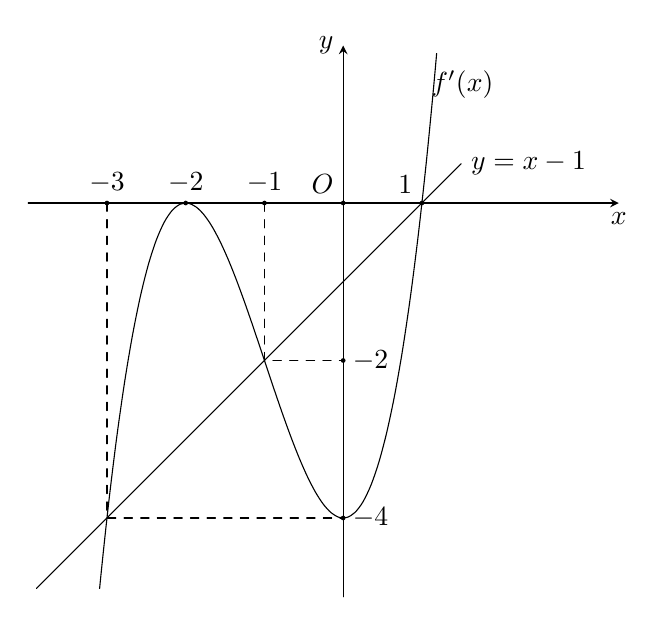
\begin{tikzpicture}[line join=round,line cap=round,>=stealth]
					\def\a{1} \def\b{3} \def\c{0} \def\d{-4} 
					\def\xmin{-4} \def\xmax{3.5} 
					\def\ymin{-5} \def\ymax{2} 
					\draw[->] (\xmin,0)--(\xmax,0)  node [below]{$x$};
					\draw[->] (0,\ymin)--(0,\ymax) node  [left]{$y$};
					\node at (0,0)  [above left]{$O$};
					 \clip (\xmin+0.1,\ymin+0.1) rectangle (\xmax-0.1,\ymax-0.1);
					\draw[smooth,samples=100] plot  (\x,{\a*(\x)^3+\b*(\x)^2+\c*(\x)+\d});
					\node at  (1,1.2) [above right]{$f’(x)$};
					\draw[dashed] (-1,0)|-(0,-2) 
						(-3,0)|-(0,-4); 
					\fill (-1,0) circle (0.03) node[above]{$-1$} 
						(0,-2) circle  (0.03) node[right]{$-2$}
						(-2,0) circle  (0.03) node[above]{$-2$}
						 (-3,0) circle (0.03) node[above]{$-3$}
						(1,0) circle (0.03) node[above left]{$1$} 
						(0,-4) circle (0.03) node[right]{$-4$} 
						(0,0) circle (0.03); 
					\draw  (-4,-5)--(1.5,0.5) node[right]{$y=x-1$};
				\end{tikzpicture}
			\end{center}
			Ta vẽ hai đồ  thị hàm số $y=f’(x)$ và $y=x-1$ trên cùng một hệ trục tọa độ.\\
			Suy ra $g’(x)=0\Leftrightarrow f’(x)-(x-1)=0  \Leftrightarrow \hoac{&x=-3\\&x=-1\\&x=1. }$\\
			Bảng biến  thiên
			\begin{center}
				
\begin{tikzpicture}
					 \tkzTabInit[nocadre,lgt=1.2,espcl=2.5,deltacl=0.6]
						{$x$  /0.6,$y'$ /0.6,$y$ /2}
						{$-\infty$,$-3$,$-1$,$1$,$+\infty$} 
					\tkzTabLine{,-,$0$,+,$0$,-,$0$,+,} 
					 \tkzTabVar{+/$+\infty$,-/$g (-3)$,+/$g (-1)$,-/$g (1)$,+/$+\infty$}
				\end{tikzpicture}
			\end{center}
			Suy ra hàm số $y=g(x)$ đồng biến  trên khoảng $(-3;-1)$ và $(1;+\infty)$.\\
			Ta thấy $\left(-\dfrac{5}{2};-\dfrac{3}{2}\right)\subset(-3;-1)$ nên  hàm số đồng biến trên $\left(-\dfrac{5}{2};-\dfrac{3}{2}\right)$.\\
		\end{itemchoice}
	} 
\end{ex}


%%%%%%%%%%%%%%%% TRẢ LỜI NGẮN %%%%%%%%%%%%%%%%

% nguồn: Phan2_Lop_12_Dai_so_Chuong_1
\begin{bt}%[2D1V5-5]%[ma:7481930e]
	Cho hàm số $y=f\left( x  \right)$ liên tục trên $\mathbb{R}$ và hàm số $y=f'\left( x \right)$ có đồ thị như hình vẽ.
	\begin{center}
		\begin{tikzpicture}[line join=round,line cap=round,>=stealth]
			\tikzset{ethicknode/.style={scale=0.9}} 
			\draw[->] (-1.1,0)--(6.1,0) node[below left] {$x$}; 
			\draw[->] (0,-1.1)--(0,6.1)  node[below left] {$y$};
			\draw  (0,0) node [below left] {$O$};
			\foreach \x/\nx in {1/x_1,3/x_2,4/x_3} 
			\draw[thin] (\x,1pt)--(\x,-1pt) node [below] {$\nx$}; 
			\foreach \y/\ny in {1/1,2/2,5/5} 
			\draw[thin]  (1pt,\y)--(-1pt,\y) node [left] {$\ny$};
			 \draw[dashed,thin](1,0)--(1,5)--(0,5);
			 \draw[dashed,thin](3,0)--(3,1)--(0,1);
			\draw[dashed,thin](4,0)--(4,2)--(0,2); 
			\begin{scope}
				\clip (-1,-1)  rectangle (6,6);
				\draw[name  path=] plot[smooth,tension=0.7] coordinates{(-1,-2)
					 (1,5)
					(3,1) 
					(4,2) 
					 (5,-1)};
			\end{scope}
		\end{tikzpicture}
	\end{center}
	Hàm số $y=f\left( x \right)+\dfrac{2017-2018x}{2017}$ có  bao nhiêu điểm cực trị?
	 \shortans{4}
	 \loigiai{
		Ta có $y'=f'(x)-\dfrac{2018}{2017}$.\\ 
		Khi đó, $y'=0\Leftrightarrow f'\left( x \right)-\dfrac{2018}{2017}=0\Leftrightarrow f'\left( x  \right)=\dfrac{2018}{2017}$.\\
		Dựa vào đồ thị, ta thấy phương trình $f'(x)=\dfrac{2018}{2017}$ có 4 nghiệm phân biệt. Do đó, hàm số đã cho có 4 điểm cực trị. 
	} 
\end{bt}
